\documentclass{beamer}
\usepackage{geometry}       
\usepackage{beamer}     
%\usetheme{Warsaw}
           % See geometry.pdf to learn the layout options. There are lots.
%\geometry{letterpaper}                   % ... or a4paper or a5paper or ... 
%\geometry{landscape}                % Activate for for rotated page geometry
\usepackage[parfill]{parskip}    % Activate to begin paragraphs with an empty line rather than an indent
\usepackage{graphicx}
\usepackage{amssymb}
\usepackage{epstopdf}

\DeclareGraphicsRule{.tif}{png}{.png}{`convert #1 `dirname #1`/`basename #1 .tif`.png}

\title{Bayesian approach for addressing covariate measurement error in propensity score methods}
\author{Elizabeth Stuart and [insert other folks here]}
\date{}                                           % Activate to display a given date or no date

\begin{document}

\begin{frame}
\titlepage
\end{frame}

\begin{frame}
\frametitle{Agenda}
\begin{enumerate}
\item Background
\begin{itemize}
\item Motivation
\item Previous Research
\item Goal
\end{itemize}
\item Methods
\begin{itemize}
\item Notation
	\item Estimands and Estimators
	\item Simulation Set-Up
\end{itemize}
\item Results
\begin{itemize}
	\item Simulation
	\item Illustrative Example
\end{itemize}
\item Conclusions
\end{enumerate}
\end{frame}

\begin{frame}
\frametitle{Motivation}

Balancing score property of propensity scores (PS) assumes that:
\begin{enumerate}
\item all confounders are observed and 
\item measured without error.
\end{enumerate}
\end{frame}

\begin{frame}
\frametitle{ Motivation}

\begin{itemize}
\item In reality, covariate measurement error may be the rule rather than the exception. 
\begin{itemize}
	\item self-reported measures: household income, weight, age of parents.
	\item imperfect instruments: blood pressure, cortisol levels.
	\item latent constructs: depression, disability.
\end{itemize}
\end{itemize}

 
\end{frame}

\begin{frame}

\frametitle{ Motivation}

\begin{itemize}
\item In reality, covariate measurement error may be the rule rather than the exception. 
\begin{itemize}
	\item self-reported measures: household income, weight, age of parents.
	\item imperfect instruments: blood pressure, cortisol levels.
	\item latent constructs: depression, disability.
\end{itemize}
\item Covariate measurement error may compromise the bias-reduction potential of propensity scores if treatment assignment depends on the true, unobserved covariate.
\end{itemize}

\end{frame} 

\begin{frame}

\frametitle{ Motivation}


\begin{itemize}
\item In reality, covariate measurement error may be the rule rather than the exception. 
\begin{itemize}
	\item self-reported measures: household income, weight, age of parents.
	\item imperfect instruments: blood pressure, cortisol levels.
	\item latent constructs: depression, disability.
\end{itemize}
\item Covariate measurement error may compromise the bias-reduction potential of propensity scores if treatment assignment depends on the true, unobserved covariate.
\item Researchers left with the choice: exclude mismeasured covariates from PS model or ignore the measurement error. 

\end{itemize}

\end{frame}

\begin{frame}
\frametitle{ Previous Research}


Focus has been on classical measurement error


$W = X + U$,  $E(U \vert X)=0$,   with constant variance $U \vert X \sim Normal(0,\sigma^2_u)$  
 

where $X$ is the correctly measured covariate, and  $W$ is the mismeasured version of $X$.

\end{frame} 

\begin{frame}

\frametitle{ Previous Research}

\begin{itemize}
\item Steiner, Cook, Shadish. 2011: Classical measurement error in covariate(s) compromises bias-reduction potential of propensity score methods.
\end{itemize}
\end{frame} 

\begin{frame}

\frametitle{ Previous Research}

\begin{itemize}
\item Steiner, Cook, Shadish. 2011: Classical measurement error in covariate(s) compromises bias-reduction potential of propensity score methods.
\item Millimet. 2010: Classical and nonclassical measurement error in covariate(s) compromises bias-reduction potential of propensity score methods. 
\end{itemize}
\end{frame} 

\begin{frame}

\frametitle{ Previous Research}

\begin{itemize}
\item Steiner, Cook, Shadish. 2011: Classical measurement error in covariate(s) compromises bias-reduction potential of propensity score methods.
\item Millimet. 2010: Classical and nonclassical measurement error in covariate(s) compromises bias-reduction potential of propensity score methods. 
\item McCaffrey, Lockwood, Setodji. 2011: Propose IPW that corrects for classical measurement error in the covariates.
\end{itemize}
\end{frame} 

\begin{frame}

\frametitle{ Previous Research}

\begin{itemize}
\item Steiner, Cook, Shadish. 2011: Classical measurement error in covariate(s) compromises bias-reduction potential of propensity score methods.
\item Millimet. 2010: Classical and nonclassical measurement error in covariate(s) compromises bias-reduction potential of propensity score methods. 
\item McCaffrey, Lockwood, Setodji. 2011: Propose IPW that corrects for classical measurement error in the covariates.
\item Lockwood, McCaffrey. 2014: Argue that PS matching using covariates measured with error (only) will not work, but suggest that using the covariates measured with error in conjunction with treatment status may work in some scenearios.
\end{itemize}
\end{frame} 

\begin{frame}

\frametitle{ Previous Research}

\begin{itemize}
\item Steiner, Cook, Shadish. 2011: Classical measurement error in covariate(s) compromises bias-reduction potential of propensity score methods.
\item Millimet. 2010: Classical and nonclassical measurement error in covariate(s) compromises bias-reduction potential of propensity score methods. 
\item McCaffrey, Lockwood, Setodji. 2011: Propose IPW that corrects for classical measurement error in the covariates.
\item Lockwood, McCaffrey. 2014: Argue that PS matching using covariates measured with error (only) will not work, but suggest that using the covariates measured with error in conjunction with treatment status may work in some scenearios.
\item Raykov. 2012: Propose latent variable approach to address covariate measurement error in propensity score methods. Assumes have congeneric measures for each covariate measured with error. 
\end{itemize}

\end{frame} 

\begin{frame}

\frametitle{ Research Gap}


Non-classical measurement error: differential by treatment status.

\begin{itemize}
\item Systematic differential measurement error that affects the mean. 
\begin{itemize}
	\item Example: Adolescents in disadvantaged neighborhoods (`treatment' group) tend to overestimate their mothers' age when the adolescents were born.
\end{itemize}
\item Heteroscedastic differential measurement error that affects the variance.
\begin{itemize}
	\item Example: Adolescents in disadvantaged neighborhoods are less accurate in knowing their mothers' age when the adolescents were born.
\end{itemize}
\end{itemize}
 

\end{frame} 

\begin{frame}

\frametitle{ Goal}


Approach that can flexibly handle covariate measurement error that is differential by treatment status.



Bayesian approach
\begin{itemize}
	\item Most flexible approach for addressing measurement error (Carroll et al., 2006). Especially useful for measurement error model involving heteroscedasticity.
	\item Propogates uncertainty.
	\item Appropriate when validation data are external to the study sample instead of internal (Cole et al., 2006).
	\item Maximum likelihood approach has similar advantages, but Bayesian is simpler to implement (Hossain, Gustafson, 2009).
\end{itemize}

 

\end{frame} 

\begin{frame}

\frametitle{ Notation}


Let observed data $O=(W, Y, A, Z)$ and complete data $C=(W, Y, A, X, Z)$, where:


\begin{itemize}
\item $Y$ = observed, continuous outcome of interest. 

\item $A$ = observed, binary (0/1) variable indicating treatment. 

\item $Z$ = observed, continuous covariate. 

\item $X$ = unobserved, continuous covariate. 

\item $W$ = observed, mismeasured version of $X$, where the mismeasurement depends on the tratment. $W \sim Normal(f(X,A), \sigma^2f(X,A)^2)$

\end{itemize}


\end{frame} 

\begin{frame}

\frametitle{ Estimand and Estimator}


Estimand: ATE 

Estimator: IPTW
\begin{itemize}
\item But, we do not observe $X$, so the ATE is not identifiable. It's possible that Bayesian models can be useful even under non-identifiability, but we need some assumptions.
\end{itemize}
\end{frame} 

\begin{frame}

\frametitle{ Estimand and Estimator}

Assumptions: 
\begin{itemize}
\item External validation data with $(A,X,W)$ that can inform priors related to measurement error.
\item External validation data generalizes to study sample.
\item $W \perp (Y, Z) \vert X, A$. Could be relaxed if $Y$ or $Z$ was observed in the validation study. 
And the usual causal inference assumptions:
\item No unmeasured confounders: for each $a \in \{ 0,1 \}$, we have $Y_a \perp A \vert X,Z$.
\item Consistency: for each $a \in \{ 0,1 \}$, we have $Y_a =Y$ on the event $A=a$.
\item Positivity: for each $a \in \{ 0,1 \}$, we have $P(A=a \vert X, Z)$ is strictly positive.
\end{itemize}

 

\end{frame} 

\begin{frame}

\frametitle{ Simulation Set-Up}


Let observed data $O=(W, Y, A, Z)$ and complete data $C=(W, Y, A, X, Z)$, where:

\begin{itemize}

\item $Y \sim Normal(3 A + 2X + 2 Z, 1)$

\item $A \sim Bernoulli(-2log(2) + log(2) \times X + log(2) \times Z)$ 

\item $Z \sim Normal(1, 1)$

\item $X \sim Normal(1 + 0.2 Z, 1)$

\item $W \sim Normal(X + 2A, 0.5(1 + A)^2)$

\end{itemize}

\end{frame} 

\begin{frame}

\frametitle{ Simulation Set-Up}

\begin{itemize}
\item Point mass priors on coefficients $(\gamma, \delta)$ in measurement error model:

$(W \vert Y, X, A, Z) \sim N(X + \gamma A, \sigma^2_{U,A=0}(1 + \delta A)^2)$

\item Strong and untestable assumption, unless internal validation data are present. 
\item Assume have external knowledge to inform priors related to measurement error.
\item Assume that this external knowledge generalizes to the study sample.
\item Non-informative priors on coefficients in treatment, outcome, and X models
\item Semi-informative priors on $\sigma_u$ and $\sigma_x$
\end{itemize}
 

\end{frame} 

\begin{frame}

\frametitle{ Simulation Results}
\centering
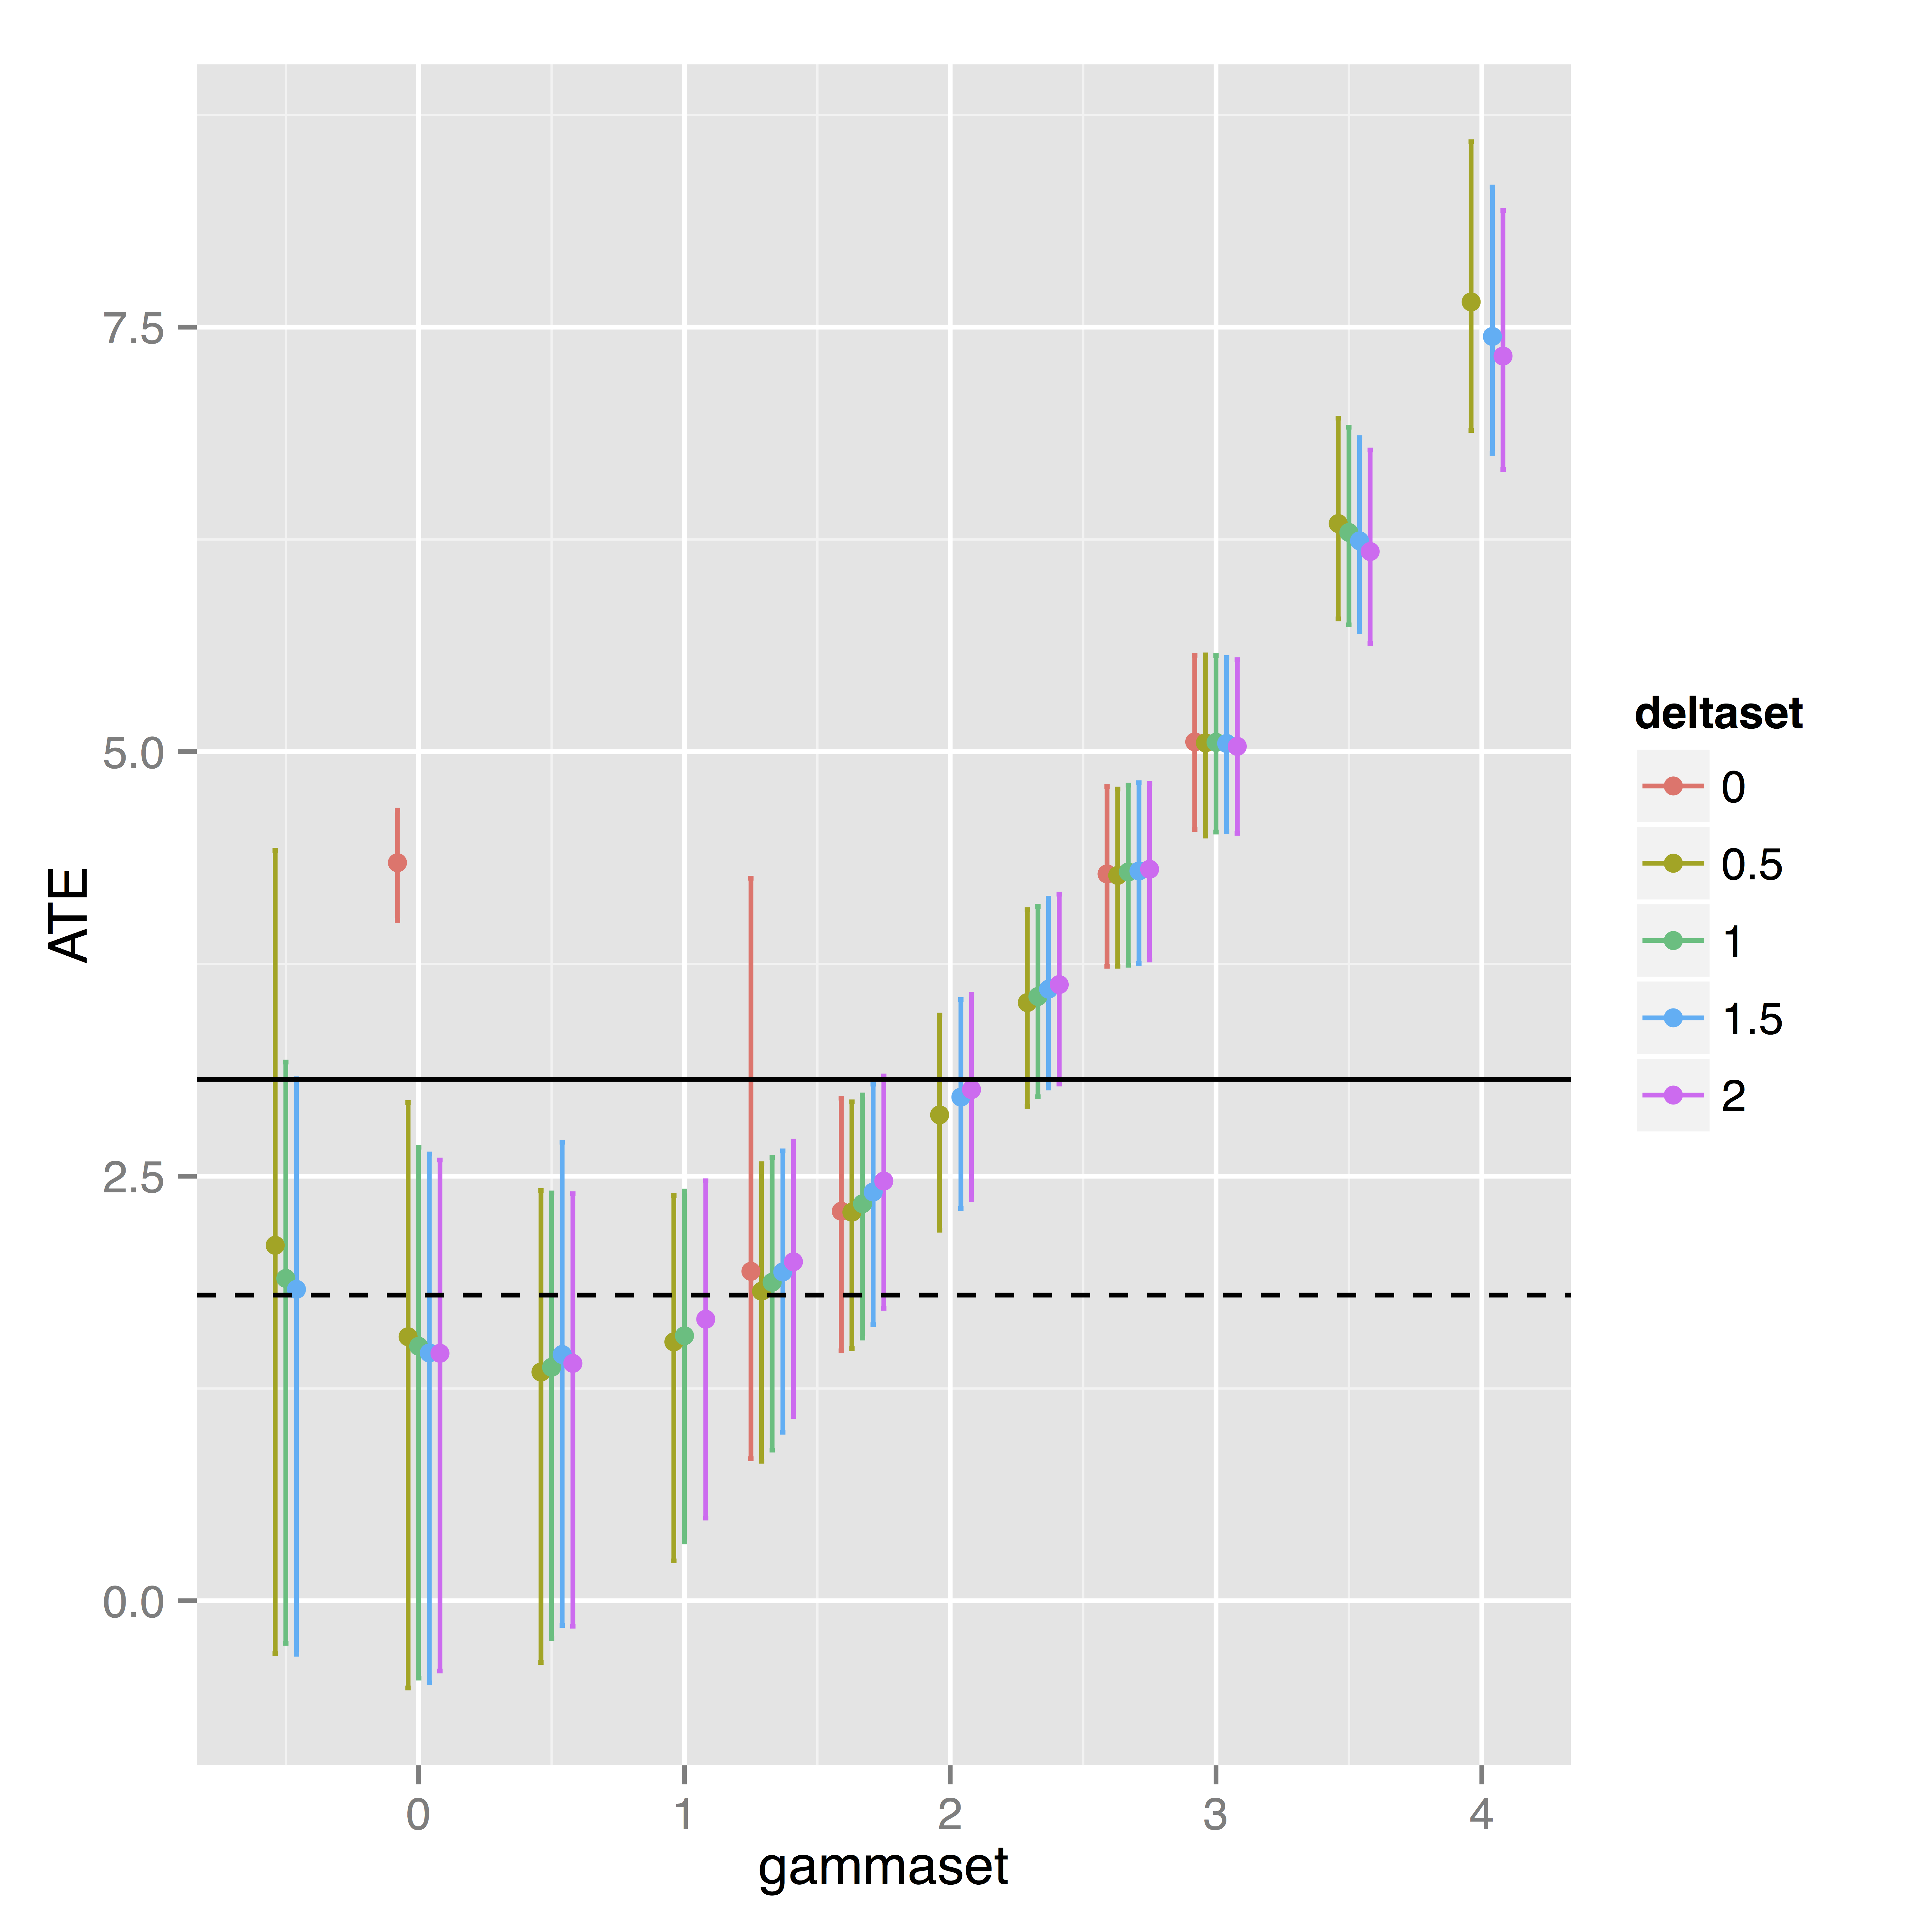
\includegraphics[width=\textwidth,height=0.9\textheight,keepaspectratio]{BayesianMESummary-007}

 

\end{frame} 

\begin{frame}

\frametitle{ Simulation Results}

\centering
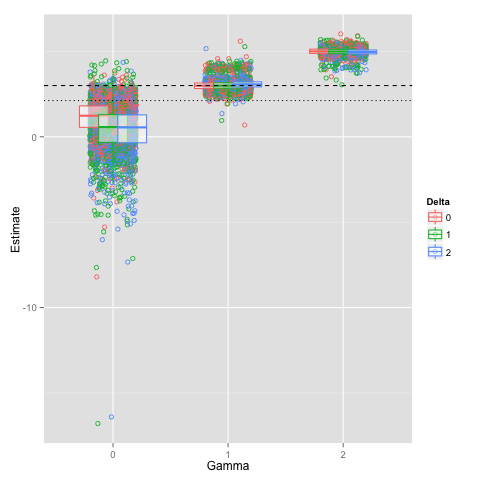
\includegraphics[width=\textwidth,height=0.9\textheight,keepaspectratio]{ATEsim}


 

\end{frame} 

\begin{frame}

\frametitle{ Simulation Results}

\begin{itemize}
\item Differential measurement error in variance (heteroscedasticity) less important than differential measurement error in the mean (agrees with Spiegelman et al., 2011).



\item Don't have to use point mass priors. Could use non-informative priors if increased the number of iterations (and therefore increase computing time).



\item Model feedback not an issue. We allow the outcome model to be a function of covariates instead of just the propensity score (as in imputation).

\end{itemize}
  

\end{frame} 

\begin{frame}

\frametitle{ Example Data}



Association between living in a disadvantaged neighborhood and past-year drug abuse or dependence disorder.

\begin{itemize}

\item Important confounders: family income, race/ethnicity, urbanicity, region of the country, age of adolescent, age of mother when the adolescent was born

\item National Comorbidity Survey Replication Adolescent Supplement: 
\begin{itemize}
	\item Nationally-representative survey of adoelscent mental health (DSM-IV diagnoses)
	\item Face-to-face, computer-assisted interviews with the adolescent. 
  	\item Self-administered questionnaire to parents or parent surrogate of the adolescent.
  	\item Geocoded residence.
\end{itemize}
\end{itemize}

\end{frame} 

\begin{frame}


\frametitle{ Example Data: Measurement Error}

\begin{itemize}

\item $X$: Mother-reported maternal age at birth 

\item $W$: Adolescent-reported maternal age at birth. Could be reported differently by neighborhood disadvantage status.
\begin{itemize}
	\item Adolescents in disadvantaged neighborhoods may think that their mothers are older than they actually are.
	\item Adolescents in disadvantaged neighborhoods may be less accurate in guessing their mother's age than adolescents in nondisadvantaged neighborhoods.
\end{itemize}
 \end{itemize}

\end{frame} 

\begin{frame}


\frametitle{ Example Data: Measurement Error}


\begin{itemize}
\item We use subset where both $X$ and $W$ are observed to evaluate how the method works.
\end{itemize}

\centering
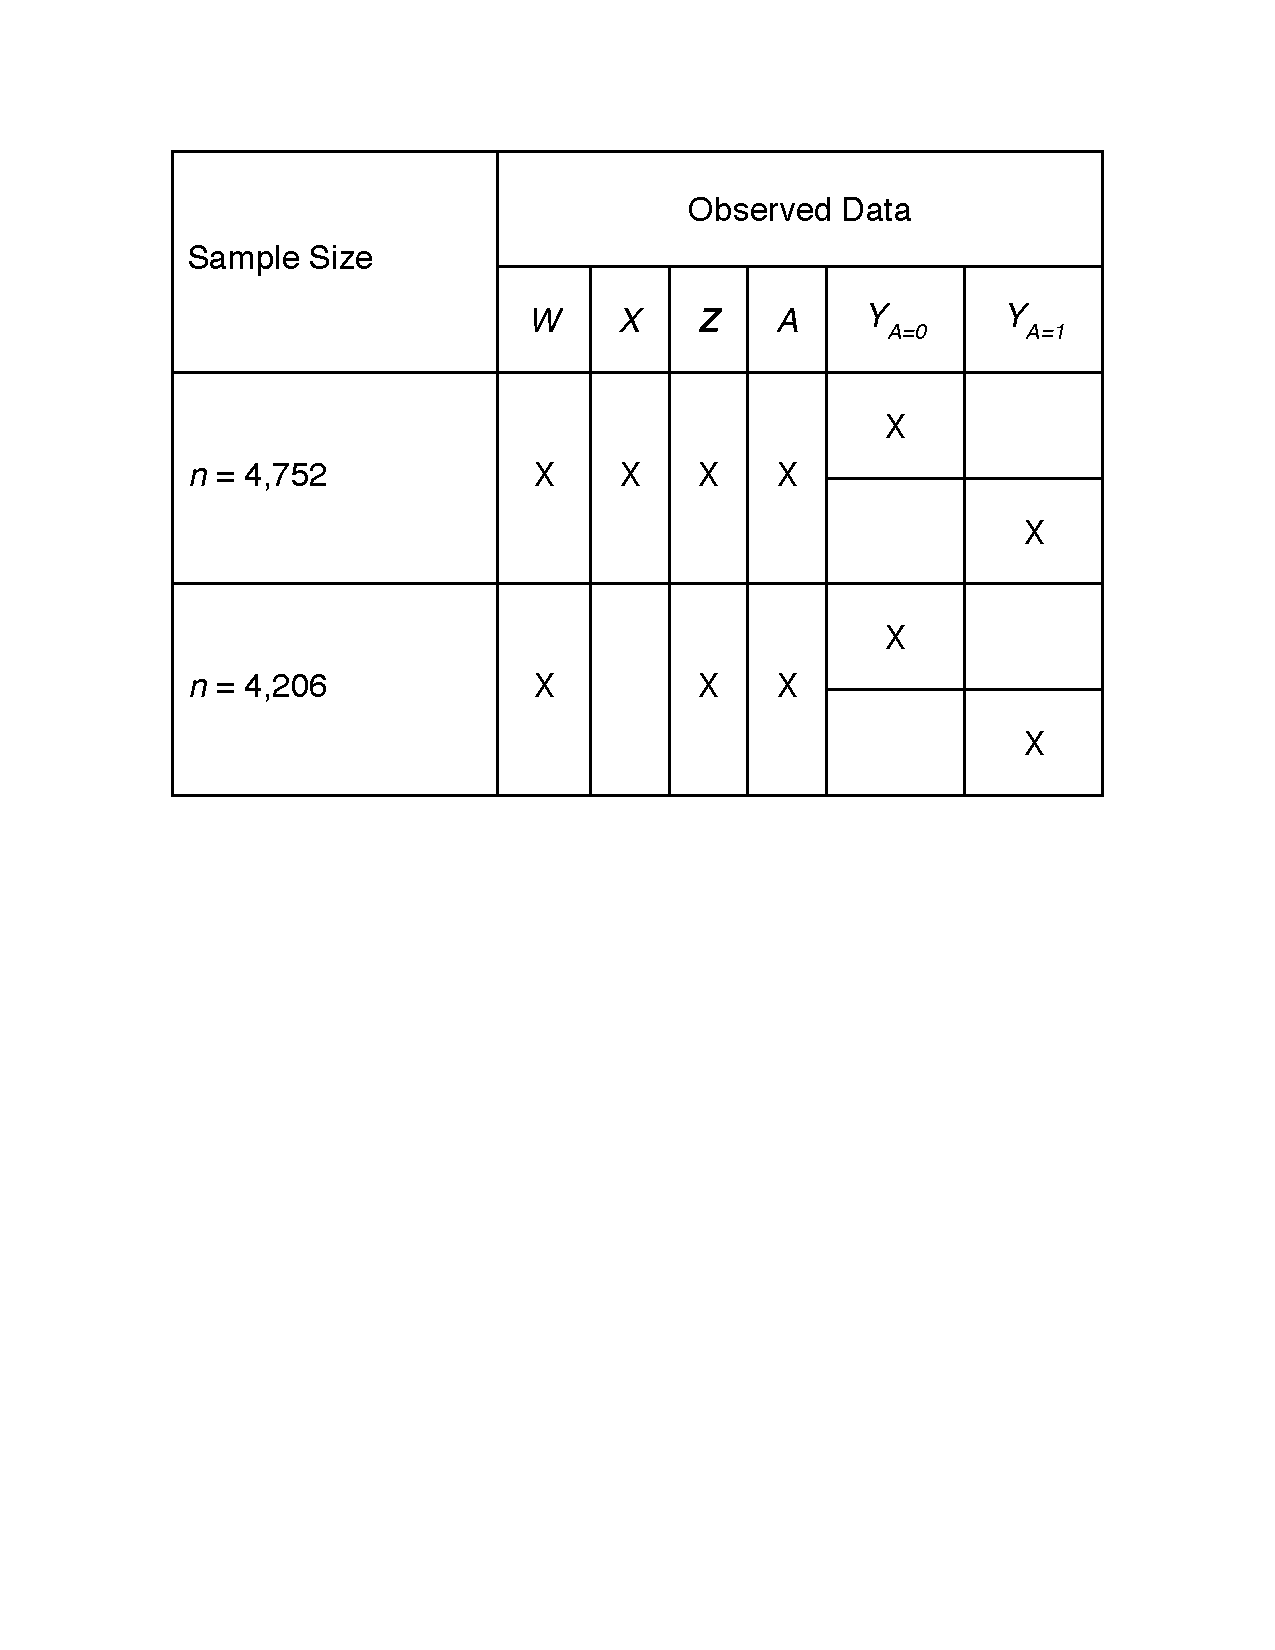
\includegraphics[width=\textwidth,height=0.7\textheight,keepaspectratio]{observeddata}


\end{frame} 

\begin{frame}

\frametitle{ Example Data: Simulated Additional Measurement Error}

We evaluate our Bayeian approach using:
\begin{itemize}
\item $W$ from the data ($\rho=0.94$)
\item $W$ with simulated additional measurement error that is differential in the location parameter ($\rho=0.7$)
\item $W$ with simulated additional measurement error that is differential in the scale parameter ($\rho=0.7$)
 \item $W$ with simulated additional measurement error that is differential in the location and scale parameters ($\rho=0.7$)
\end{itemize}
 


\end{frame} 

\begin{frame}

\frametitle{ Example Data: Results}

$W$ with simulated additional measurement error that is differential in the location parameter ($\rho=0.7$)

\centering
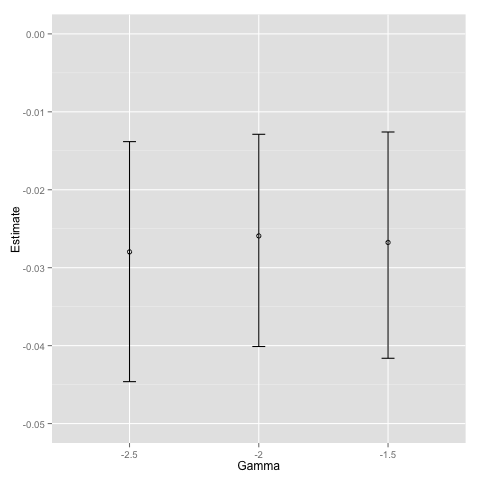
\includegraphics[width=\textwidth,height=0.7\textheight,keepaspectratio]{gammarealdatamini}

 

\end{frame} 

\begin{frame}

\frametitle{ Example Data: Results}

$W$ with simulated additional measurement error that is differential in the scale parameter ($\rho=0.7$)

\centering
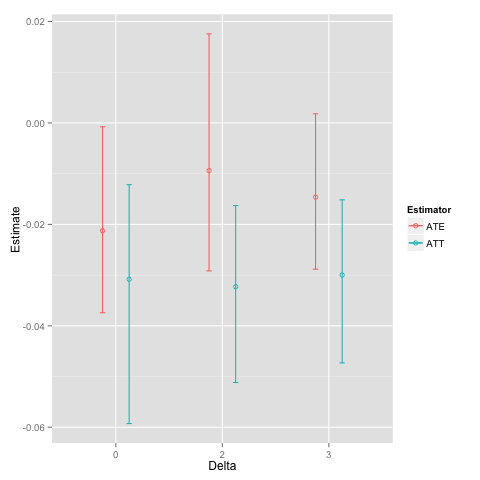
\includegraphics[width=\textwidth,height=0.7\textheight,keepaspectratio]{deltarealdatamini}

 

\end{frame} 

\begin{frame}

\frametitle{ Example Data: Results}

$W$ with simulated additional measurement error that is differential in the location and scale parameters ($\rho=0.7$)


[insert figure]

 

\end{frame} 

\begin{frame}

\frametitle{ Future Work}



\end{frame} 

\begin{frame}

\frametitle{ Conclusions}

\end{frame}
  


\end{document}
